%% use JSS class -- use 'nojss' to turn off header
\documentclass[shortnames,nojss,article]{jss}
\usepackage{booktabs,flafter,thumbpdf}
%\VignetteIndexEntry{cpda-introduction}


\author{Yi-Shin Lin\\University of Tasmania \And
Andrew Heathcote\\University of Tasmania \And
William R. Holmes\\Vanderbilt University}
\Plainauthor{Yi-Shin Lin, Andrew Heathcote, William Holmes}

\title{\proglang{cpda} and \proglang{gpda}: Efficient Computation for
Probability Density Approximation}
\Plaintitle{A Solution for Efficient Computation
of Probability Density Approximation}

\Abstract{
  Probability density approximation (PDA) efficiently calculates
  likelihood even when their analytic functions are unavailable.  It
  allows researchers to model compuationally complex biological processes,
  which in the past could only be approached by overly simplified
  models. It is however computationally demanding.  We implement two
  \proglang{R} packges, \pkg{cpda} and \pkg{gpda}, using
  \proglang{Armadillo C++}
  and \proglang{CUDA C} to provide a practical and efficient solution
  for Bayesian computation of cognitive models. Both packages
  harness the multi-thread nature of modern computational processing units,
  enabling parallel computations with a dozens of cores of central processing
  unit (CPU) and thoudands threads of graphics processing unit (GPU).
  \pkg{cpda}
  resolves the bottleneck when few fast CPU cores are efficient to find
  optimal solutions, such running multiple Markov chains in parallel, whereas
  \pkg{gpda} reduces the computation times when large numbers (>1e5) of Monte
  Carlo simulations is required to approximate probability densities. We 
  conclude with three practical exmaples as a road map for the application in 
  cognitive models.
}

\Keywords{\proglang{R}, \proglang{C++}, \proglang{GPU}, kernel density estimate,
Markov Chain Monte Carlo, Fourier-based PDA}
\Plainkeywords{R, C++, GPU, kernel density estimate, Markov Chain Monte Carlo}

\Volume{40}
\Issue{8}
\Month{April}
\Year{2011}
\Submitdate{2010-11-15}
\Acceptdate{2011-03-21}

\Address{
  Yi-Shin Lin\\
  Division of Psychology, School of Medicine\\
  University of Tasmania \\
  Private Bag 30 Hobart TAS 7005,\\
  Australia\\
  E-mail: \email{yishin.lin@utas.edu.au}\\
  URL: \url{http://www.tascl.org/yi-shin-lin.html}

  Andrew Heathcote\\
  School of Psychology,
  University of Newcastle\\
  Psychology Building,
  University Avenue, Callaghan, 2308,NSW, Australia\\
  E-mail: \email{andrew.heathcote@newcastle.edu.au}\\
  URL: \url{http://www.newcl.org/Heathcote/}

  William Holmes\\
  Department of Physics and Astronomy,
  Vanderbilt University\\
  Nashville, TN 37212, United States of America\\
  E-mail: \email{william.holmes@vanderbilt.edu}\\
}

%% need no \usepackage{Sweave.sty}

%


\begin{document}

\vspace*{.25cm}

\section{Introduction}
\label{sec:intro}
Simulation-based algorithms recently find a new
application in finding likelihood functions \citep{sisson_likelihood_2010}.
This application is especially useful when specifying a likelihood function 
analytically is unlikely or
when evaluating it is computationally prohibitive, a situation
arises sometimes in cognitive and often in neuro-cognitive models. These
algorithms are often referred to as \textit{likelihood-free computation} or
\textit{approximate Bayesian computation} (ABC) \citep{sisson_likelihood_2010}.
Probability density approximation (PDA) is one such
method. Unlike other likelihood-free methods, it
circumvents the difficulty of identifying sufficient summary statistics,
a set of numbers supplying as much information for data as unknown model
parameters \citep{turner_generalized_2014} by processing the data directly. This is
crucial, because it is often unlikely to know whether a set of summary
statistics is sufficient when its likelihood function is unavailable.

Because of its non-parameteric nature, PDA however suffers two computation
bottlenecks.  First is calculating kernel density estimates (KDE) for every
data point and second is conducting Monte Carlo (MC) simulations.
The computation problem is aggravated when applying PDA in Bayesian modeling,
because KDE and MC simulations are conducted iteratively in
multiple Markov chains. More importantly, the bottlenecks not only incur
computation burdens, but also
closely relate to computation errors, which have to be minimized
\citep{turner_generalized_2014}. Hence an efficient computation method is critical
not just for reducing time, but also for minimizing errors.

\cite{holmes_practical_2015} derived a fast Fourier-based algorithm, named resampled PDA
(R-PDA), to reduce computation steps, and thereby to mitigate the first
bottleneck.  In short, R-PDA transfers KDE to spectrum domains, rendering
convolution
to multiplication operations. R-PDA thereby greatly decreases
computation costs and potential errors in the first bottleneck. The second
bottleneck however is largely unresolved. Here we present software for
efficient PDA and R-PDA computations (Holmes, 2015; Turner \& Sederberg, 2014),
and resolve the second bottleneck by applying three recent computational
techniques.

First, we code PDA in \proglang{Armadillo C++}, a high efficient \proglang{C++}
library for linear algebra (Sanderson \& Curtin, 2016). Second, we implement
\proglang{Open MP} to harness multiple-core CPU, as it has become commonplace
with a regular personal computer (PC) equipping at least 4 cores in a central
process unit (CPU). Third, we implement PDA also in Compute Unified Device
Architecture, \proglang{CUDA}, a programming model recognizing the structure of
graphics processing unit (GPU); hence, \pkg{gpda}\footnote{\proglang{gpda}
stands for GPGPU-based PDA. Similarly \proglang{cpda} stands for C++-based PDA}
package allows a regular PC user to enjoy computation power of thousands GPU
cores.

To ease the installation and usage of the packages, we take advantage of the
infrastructure of the Comprehensive \proglang{R} Archive Network (CRAN).
Specifically, \pkg{cpda} and \pkg{gpda} conform CRAN standard and available at
\url{http://CRAN.R-project.org/package=cpda} and
\url{http://CRAN.R-project.org/package=gpda} with numerous examples in their
help pages. The user can easily install the packages using the
\proglang{install.packages} function in R or GUI interface, such as the one
provided by R GUI or \textit{RStudio}.

\makeatletter
\if@nojss
  This vignette corresponds to the paper published in the \textsl{Journal of
    Statistical Software}. It is currently still identical to
  the published paper.  Over time, this vignette version may receive minor
  updates. This version corresponds to \pkg{cpda} version 0.0.2.1 and was
  typeset on March 29, 2017.
\fi
\makeatother


\subsection{Four Simple Examples}
We illustrate four examples, using \pkg{cpda} to construct
simulated probability density functions (SPDFs). First example reconstructs
the starnard Gaussian distribution. Because the Gaussian distribution has an
analytic probability density function (PDF), we can easily verify whether the
SPDF generated by \pkg{cpda} successfully approximates the analytic PDF.

%
\begin{Code}
require(cpda)
n      <- 1e5                        ## Number of simulations
x      <- seq(-3,3, length.out=100)  ## Support
xlabel <- "Observations"
ylabel <- "Density"

## Simulate Gaussian distribution -----------
sam  <- rnorm(n)                     ## Monte Carlo simulations
den1 <- cpda::logLik_pw(x, sam)      ## PDA
den2 <- logLik_fft2(x, sam)          ## R-PDA
den3 <- dnorm(x)                     ## Analytic Gaussian likelihood

## Verify the three methods converge to the same PDF
png(file="doc/gaussian.png", width=800, height=600)
par(mar=c(4,5.3,0.82,1))
plot(x, exp(den1), type="l", lty="dotted", xlab=xlabel, ylab=ylabel, cex.lab=3,
  cex.axis=1.5, lwd=3)
lines(x, exp(den2[,2]), col="blue", lty="dashed", lwd=2)
lines(x, den3, col="red", lwd=2)
dev.off()
\end{Code}
%

\code{logLik_pw} returns point-wise log-likelihood. It uses PDA to calculate
log-likelihood for each observation.  It takes
about 0.323 second to get SPDF with 100,000 simulations. Using R-PDA
(Holmes, 2015), we can further reduce computation times. This is useful for the
case where observations share the same parameters.

%
\begin{Code}
system.time(den2 <- logLik_fft2(x, sam)
##  user  system elapsed
## 0.124   0.000   0.122

head(den2)
##           [,1]      [,2]
## [1,] -3.000000 -5.420678
## [2,] -2.939394 -5.240477
## [3,] -2.878788 -5.048910
## [4,] -2.818182 -4.850126
## [5,] -2.757576 -4.671268
## [6,] -2.696970 -4.498645
\end{Code}
%

\code{logLik_fft2} takes only 0.122 second return a SPDF.  It is about
2.6 times faster than \code{logLik_pw}.  It returns a matrix with the
first column storing the data (ie \code{x}) and the second column storing
log-likelihood.

The three density solutions,  \code{logLik_fft2}, \code{logLik_pw}, and
analytic Gaussian function, match one another, as shown by the overlapping
density curves (Figure~\ref{fig:gaussian}).

\begin{figure}[htbp]
\begin{center}
    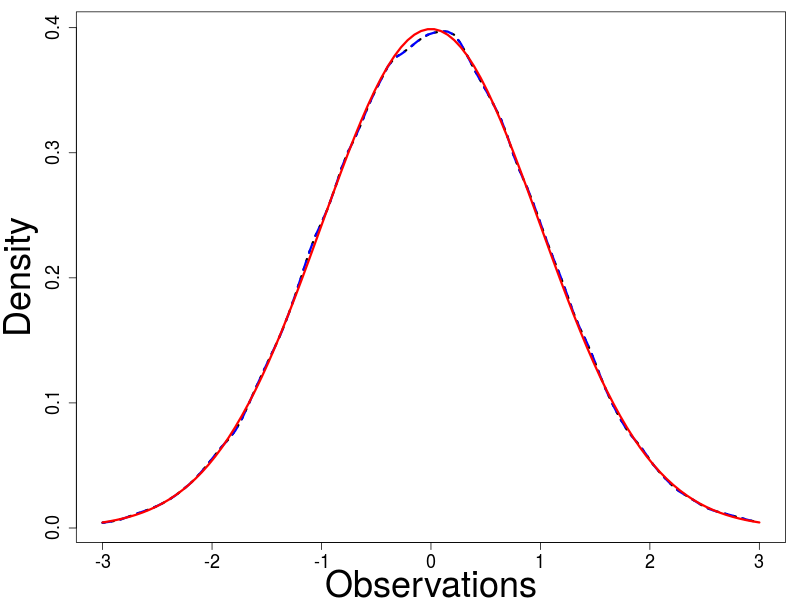
\includegraphics[width=0.5\textwidth]{figs/gaussian}
      \caption{Three solutions for the Gaussian density function. The black,
      blue and red curves are on top of one another.}
      \label{fig:gaussian}
\end{center}
\end{figure}

PDA is a general method, working also for other distributions. The
following example demonstrates approximating the probabilities of an exponential
modified Gaussian (ex-Gaussian) distribution, a standard distribution being
used often to describe response time data \citep{dawson_fitting_1988}. Again, becasue
ex-Gaussian distribution has an analytic form, we can verfiy resampled PDA
successfully recover likelihood.

%
\begin{Code}
## Simulate ex-Gaussian distribution -----------
## We used the rexGAUS function in gamlss.dist package, downloaded from
## https://cran.r-project.org/web/packages/gamlss.dist/index.html
## Simulate ex-Gaussian distribution -----------
n    <- 1e5
sam  <- gamlss.dist::rexGAUS(n, mu=0, sigma=1, nu=1)
x    <- seq(-4, 4, length.out=100) ## Support
den1 <- cpda::logLik_pw(x, sam)
den2 <- logLik_fft2(x, sam)
den3 <- gamlss.dist::dexGAUS(x, mu=0, sigma=1, nu=1)

xlabel <- "Observations"
ylabel <- "Density"


png(file="doc/exG.png", width=800, height=600)
par(mar=c(4,5.3,0.82,1))
plot(x, exp(den1), col="grey", type="l", lty="dotted", xlab=xlabel, ylab=ylabel,
  cex.lab=3, cex.axis=1.5, lwd=3)
lines(x, exp(den2[,2]), lty="dashed", lwd=3)
lines(x, den3, col="red", lwd=3)
dev.off()

\end{Code}
%

\begin{figure}[htbp]
\begin{center}
    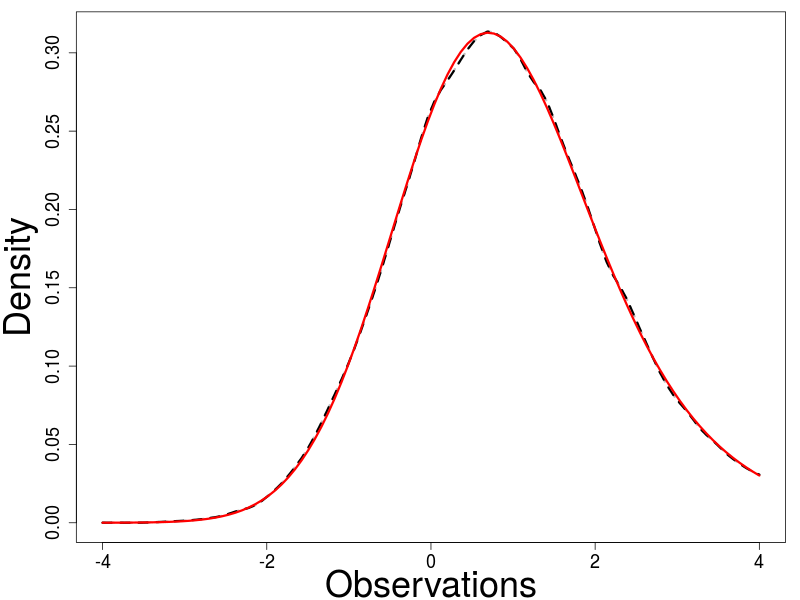
\includegraphics[width=0.5\textwidth]{figs/exG}
      \caption{Approximating exponential modified Gaussian distribution.}
      \label{fig:exG}
\end{center}
\end{figure}

Figure~\ref{fig:exG} shows PDA, R-PDA and analytic ex-Gaussian density
function return almost identical likelihood.

The next example demonstrates an interesting application, using
a slightly complicated example. We use PDA to recover probabilities from a
regression model, $ y = ax + b + \epsilon $. This is the case where the
parameters for each data point differ.

Because each data point is sampled from a Gaussian distribution
with a different mean, we need to conduct simulations separately for each of 
them. We can use R's sapply function or even better C++ iterator to speed up 
the compuation. To make code more readable, we wrote it in a simple for loop 
here.

%
\begin{Code}
n      <- 1e5
x      <- seq(-3, 3, length.out=100) ## Support
xlabel <- "x"
ylabel <- "Density"
theta  <- c(a=7.5, b=3.5, s=5)       ## slope, intercept and sigma
y      <- rnorm(length(x), mean=theta[2]+theta[1]*x, sd=theta[3])
dat    <- cbind(x, y)
den1   <- numeric(length(x))         ## a container to store likelihood

## Even we simulate for each data point, it takes cpda only 2 seconds with
## 100 x 1e5 simulations
##   user  system elapsed
##  2.084   0.004   2.087
for(i in 1:length(x)) {
  sam     <- rnorm(n, theta[2]+theta[1]*x[i], theta[3])
  den1[i] <- cpda::logLik_pw(x[i], sam)
}

## Get analytic likelihood
den2 <- dnorm(x, theta[2]+theta[1]*x, theta[3])


png(file="doc/regression.png", width=800, height=600)
par(mfrow=c(1,2))
par(mar=c(4,5.3,0.82,1))
plot(x,y, cex.lab=3, cex.axis=1.5, lwd=3)
plot(x, exp(den1),  col="grey", type="l", lty="dotted", xlab=xlabel,
  ylab=ylabel, cex.lab=3, cex.axis=1.5, lwd=3)
lines(x, den2, lwd=3, lty="dashed")
dev.off()

\end{Code}
%

\begin{figure}[htbp]
\begin{center}
    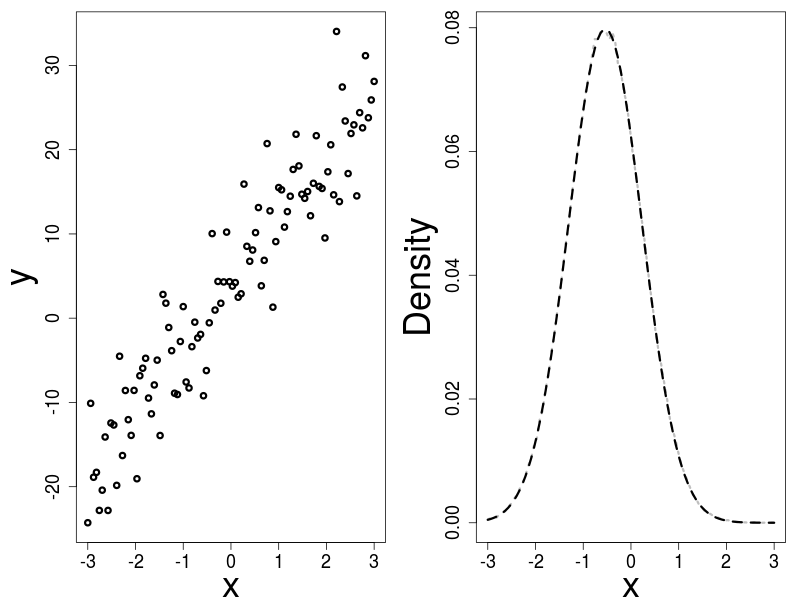
\includegraphics[width=0.65\textwidth]{figs/regression}
      \caption{Regression data and their likelihood approximation. The
      approximated solution is almost identical to the analytic solution,
      so the grey and drak lines are hardly distinguishable.}
      \label{fig:regression}
\end{center}
\end{figure}


The last example, linear ballistic accumulation (LBA) model, is a simplified
evidence accumulation model \citep{brown_simplest_2008}. The model
accounts for the data of choice response time (RT), often collected in a
psychological experiment where a participant make a speedy choice for multiple
alternatives.  In the case of two-choice task, a data point consists of a
response time and a choice (e.g., choice 1 made by .800 second).


\begin{Code}
## Simulate linear ballistic accumulator distribution -----------
## We use the "rLBA" function in rtdists to generate "empirical" data, which
## have 1,000 choice RT responses.
## rtdists can be downloaded at:
## https://cran.r-project.org/web/packages/rtdists/index.html
y <- rtdists::rLBA(1e3, A=.5, b=1, t0=.25, mean_v=c(2.4, 1.2), sd_v=c(1, 0.6))
y1 <- sort(y[y$response==1, "rt"]) ## rt1
y2 <- sort(y[y$response==2, "rt"]) ## rt2  
\end{Code}
%

The empirical RT distributions for choice 1 and choice 2 skew towards
positive side, where fast responses are truncated and slow responses are
infrequent. Because the analytic LBA PDF is known, we can calculate it directly
using the equation provided in \citep{brown_simplest_2008}.

\begin{Code}
den0 <- rtdists::dLBA(y$rt, y$response, A=.5, b=1, t0=.25, mean_v=c(2.4, 1.2), 
  sd_v=c(1, .6))
df0  <- cbind(y, den0)
df1  <- df0[df0[,2]==1,]
df2  <- df0[df0[,2]==2,]
den1 <- df1[order(df1[,1]),3]
den2 <- df2[order(df2[,1]),3]

\end{Code}
%


\begin{figure}[htbp]
\begin{center}
    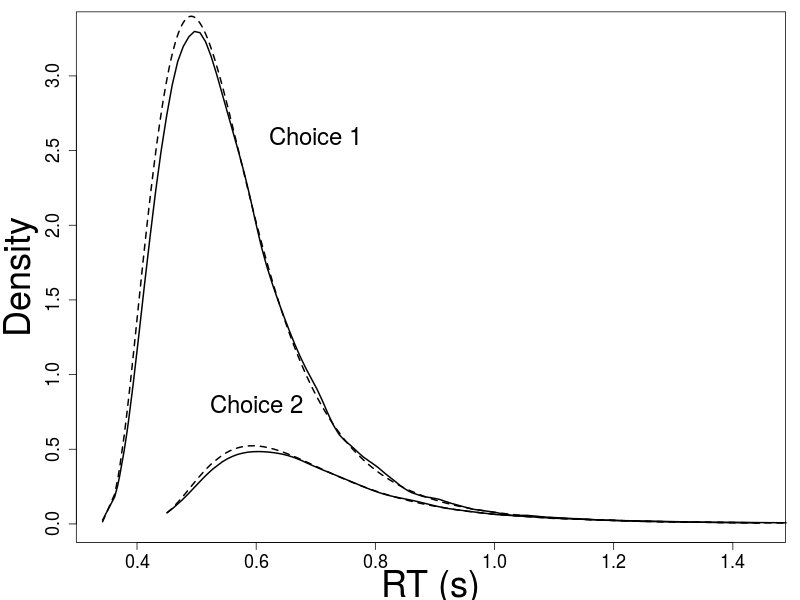
\includegraphics[width=0.65\textwidth]{figs/lba-pda}
      \caption{The solid and dashed lines show empirical and simulated
      probability density function, respectively. The empirical data were
      generated with the following parameters: upper bound for the starting
      evidence, $A=.5$, response threshold, $b=1$, non-decisoin time $t0=.25$,
      mean drift rates for accumulator \textit{1} and accumulator \textit{2},
      $(2.4, 1.2)$, and their standard deviations, $(1, 0.6)$.}
      \label{fig:lba-pda}
\end{center}
\end{figure}

Even though there is an analytic solution for its probability density
function \citep{brown_simplest_2008}, we assume for now the density function is
not available. Therefore, we used PDA to find SPDF as an alternative solution
for the density function. A cannoical LBA model samples a starting value for
sensory evidence stochastically from a uniform distribution with bounds, 0 and
$A$ and a rate of evidence accumulation (i.e., drift rate) from a Gaussian
distribution. To eliminate the possibility of negative drift rate, we sampled
drift rates from a truncated normal distribution. This LBA theory enables us
to conduct Monte Carlo simulations of LBA model without knowing its PDF.


\begin{Code}
n    <- 1e5          ## the size of simulated sample
pVec <- c(A1=1, A2=1, b1=.5, b2=.5, v1=2.4, v2=1.2, sv1=1, sv2=.6, 
          t01=.25, t02=.25)

## Monte Carlo simulations for choice 1 and 2
samp  <- cpda::rlba(n, pVec)
samp1 <- samp[samp[,2]==1, 1]
samp2 <- samp[samp[,2]==2, 1]

## Use R-PDA to estimate densities. Because each choice is defective,  
## the user needs to indicate the total number of simulated samples. 
system.time(fft1 <- cpda::logLik_fft2(y1, samp1, n=n))
system.time(fft2 <- cpda::logLik_fft2(y2, samp2, n=n))

## Use PDA to estimate densities. Again considering defective.
system.time(fft3 <- cpda::logLik_pw(y1, samp1, n=n))
system.time(fft4 <- cpda::logLik_pw(y2, samp2, n=n))

## Use Open MP to speed up piecewise computation
system.time(fft5 <- cpda::logLik_pw(y1, samp1, n=n, parallel=T))
system.time(fft6 <- cpda::logLik_pw(y2, samp2, n=n, parallel=T))

## ny1=828; nsamp1=81164
## 0.024   0.004   0.026   ## logLik_fft
## 1.568   0.004   1.568   ## logLik_pw
## 10.220  0.000   0.905   ## logLik_pw with parallel=T 12 cores

\end{Code}
%


\begin{Code}
xlabel <- "RT (s)"
ylabel <- "Density"

par(mar=c(4,5.3,0.82,1))
plot(y1, exp(fft1[,2]), type="l", xlab=xlabel, ylab=ylabel, cex.lab=3, 
     cex.axis=1.5, lwd=2)
lines(y2, exp(fft2[,2]), lwd=2)
lines(y1, exp(fft3), lty="longdash", lwd=2)
lines(y2, exp(fft4), lty="longdash", lwd=2)
lines(y1, exp(fft5), lty="dotted", lwd=2)
lines(y2, exp(fft6), lty="dotted", lwd=2)

lines(y1, den1, lty="dashed", lwd=2)
lines(y2, den2, lty="dashed", lwd=2)

text(0.7, 2.6, "Choice 1", cex=2)
text(.85,  0.8, "Choice 2", cex=2)
dev.off()
\end{Code}
%

SPDFs for choice 1 and choice 2 are almost indistinguishable from the analytic 
PDF (Figure \ref{fig:lba-pda}).


\subsection{Probability Density Approximation}
In this section, we gave an overview of PDA and its
enhancement, resampled PDA.  Interested readers can find an exposition in
\cite{turner_generalized_2014} for PDA and further elaboration about how
resampled PDA improves PDA in \cite{holmes_practical_2015}. Good reviews of ABC
can be found in \cite{sisson_likelihood_2010} and \cite{beaumont_approximate_2010}.

Bayesian inference derives the postioer distribution defined by a set of model
parameters via multiplying a \textit{prior} distribution, $\pi(\theta)$, by a
model likelihood function, $\pi(y|\theta)$. This is described by the
well-known Bayes' theorem:

\begin{equation} \label{eq:1}
\pi(\theta|y)=\frac{\pi(y|\theta)\pi(\theta)}{\int{\pi(y|\theta)\pi(\theta)d\theta}}
\end{equation}

More often, Bayes's theorem is processed proportionally, because the denominator
in the equation \ref{eq:1} is a constant.

\begin{equation} \label{eq:2}
\pi(\theta|y) \propto \pi(y|\theta)\pi(\theta)
\end{equation}

On the left hand side of the equation \ref{eq:2}, $\pi(\theta|y)$ stands for
the posterior probability densitiy function for a set of model parameters,
$\theta$, conditional on a given data set $y$. Both $\theta$ and $y$ can be a
scalar or a vector. The first term on the right hand side is
the likelihood function conditional on
the $\theta$. The second term is the prior probability density function for the
$\theta$, which often is chosen arbitrarily.

In a standard Bayesian inference, one first proposes a set of
parameters, often denoted $\theta^{*}$. There are a number of ways to propose parameters. A
traditional method is to sample from a jumping distribution
\citep{gelman_bayesian_2014}, but other elaborated methods are also available, such as
No-U-turn sampler \citep{hoffman2014_nut} and DE-MCMC sampler 
\citep{Braak2006,Turner2013}.  Together with an
empirical data set, one can derive a posterior probability density based on
proposal parameters simply by calculating the right hand side of the equation
\ref{eq:2}.  This proposal density is then compared to a reference
density, for example in a Markov chain, the density in a previous iteration.  This
comparison is usually a ratio of the proposal density to the reference
density, so the constant term in equation \ref{eq:1} can be safely ignored.
The ratio, $\frac{\pi(\theta^{*}|y)}{\pi(\theta^{i-1}|y)}$, is then subjected
to an accept-reject, such as Metropolis, algorithm to
decide whether the proposed or the reference paraemters is more probable in
light of given data, and thereby accepted (or rejected, if less probable).

The problem PDA, and generally ABC, tackle is the situation when the analytic
form of $\pi(y|\theta)$, is difficult to derive.  When the analytic
likelihood is unavailable, a standard Bayesian inference becomes impossible to
process.

PDA replaces $\pi(y|\theta)$ with a weighting function, $\pi(y|x, \theta)$,
multiplying a SPDF, $\pi(x|\theta)$. $x$ represents simulated data. This
renders the posterior probability density function:

\begin{equation} \label{eq:3}
\hat{\pi}(\theta|y) \propto \pi(y|x,\theta)\pi(x|\theta) \pi(\theta)
\end{equation}

So when the analytic likelihood function, $\pi(y|\theta)$, is
unavailable, one can still approximate probability densities, namely SPDF, via
Monte Carlo simulations as long as a theoretical model can be prescribed,
such as the LBA example in previous section.  In PDA, the weighting
function, $\pi(y|x, \theta)$, could be a standard Gaussian, a
Epanechnikov  \citep{holmes_practical_2015,turner_generalized_2014}, or
any other kernel function:

\begin{equation} \label{eq:4}
K_h(z) = \frac{1}{h}K(\frac{z}{h})
\end{equation}

$z$ is the discrepancy between an empirical datum and a simulate datum
($y-x_j$ in the following equation). $K$ is the kernel funciton. Replacing the
smoothing kernel into equation \ref{eq:3}, we can then derive
the equation of the weighting function mulitplying SPDF (namely, weighted SPDF): 

\begin{equation} \label{eq:5}
\hat{f}(x) = \frac{1}{N_s} \sum^{N_s}_{j=1} K_h (y-x_j)
\end{equation}

$N_s$ is the number of MC simulations, used to construct SPDF. $h$ is the
bandwidth of the kernel. Bandwidth determines the degree to which one wishes 
to smooth the kernel \citep{silverman_density_1986}. The larger the bandwidth, 
the more smoothing is appled on simulated data.

R-PDA harnesses the fact that the right hand side of equation \ref{eq:5}
equals to convolution operations of SPDF and the kernel function, and
convolutions are computationally intensive.  It is a common practice
in signal processing to transform signals in the time domain to the frequency
domain.

\begin{equation} \label{eq:6}
\hat{f}(x) = \pi(x|\theta) \star K_h(z)
\end{equation}

R-PDA applies exactly the same technique, transforming both SPDF and
kernel function to the frequency domain, conducting mulitplication operations
and transforming the result back. Hence, an efficent way to derive (weighted)
approximated probability densities is:

\begin{equation} \label{eq:7}
\hat{f}(x) = \mathcal{F}^{-1}(\mathcal{F}[\tilde{d}] \cdot  \mathcal{F}[K_h])
\end{equation}

$\mathcal{F}$ and $\mathcal{F}^{-1}$ stand for fast-Fourier transformation
(FFT) and inverse FFT operations. $\tilde{d}$ is SPDF.  Here, we use the 
canonical Gaussian kernel, utilizing its nature that a Fourier transformed 
Gaussian is another Gaussian \citep{holmes_practical_2015}.

\section{Implementation}

Both \pkg{cpda} and \pkg{gpda} were written in \proglang{C++}.  The latter 
conducts FFT operations at the GPU by writing \code{logLik_fft} 
function in \proglang{CUDA C}. Both packages implement three main functions 
\code{logLik_pw}, \code{logLik_fft}, and \code{logLik_fft2} to calculate 
model likelihood. The first function implements equation \ref{eq:5} and the 
latter two implement equation \ref{eq:7}.  Although equation \ref{eq:7} is 
faster than equation \ref{eq:5}, there are occassions, such as the regression 
example in Section \ref{sec:intro}, when the likelihood for each observation is 
based on MC simulations with their own parameter set.  

The difference between \code{logLik_fft} and \code{logLik_fft2} is
that the former returns a summed log-likelihood value, and the latter returns 
a matrix with first column orderd observations and second column storing their
log-likelihood values. 

Specifically, \code{logLik_pw} takes five arguments:

\begin{enumerate}
\item \code{y}: a vector storing empirical observations 
\item \code{yhat}: a vector storing simulations
\item \code{h}: a scalar, indicating the kernel bandwidth. 
\item \code{m}: a scalar, a multiplier to adjust bandwidth proportionally 
\item \code{parallel}: a logical switch to run parallel computing with multiple 
CPU cores. When the switch is on, \code{logLik_pw} distributes simulated 
data to available CPU cores to calculate equation \ref{eq:4} in parallel. 
\end{enumerate}

\code{logLik_pw} returns logged likelihood for each observation corresponding 
to the input vector, \code{y}.  

Similarly, \code{logLik_fft} and \code{logLik_fft2} take also \code{y}, 
\code{yhat}, \code{h} and \code{m} arguments. They take also three other 
arguments: 

\begin{enumerate}
\item \code{p}: adjusting grid size for the SPDF as a power of 2. 
\item \code{ns}: the number of simulated samples  
\item \code{defected}: a boolean switch to use \code{ns} when approximating 
defected densities.
\end{enumerate}

\section{A Real-world Example}
\label{sec:rwexample}

Piecewise linear ballistic accumulator model (PLBA) is a cognitive model, 
accounting for the decision process when one evaluates changing information 
pertinent to a decision.  For example, on a motor way, a motorist may want 
to drive as fast as permited to save journey time, and also to maintain a 
safe distance from its preceding vehicle.  In simple term, the relevant 
information is the
distance between the two vehicles, which influences the motorist's decision to
accelerate or decelerate.  The relatively stable decision information may 
abruptly change, when for example another vehicle switches lane and the 
original information favoring accelerating suddenly becomes the other way 
around.

PLBA uses LBA model as a building block to account for this type of decision 
making process.  Because of the abrupt information switching and unknown 
cognitive processes that may happen during the switching, it is less 
straighforward to derive an analytic likelihood function for PLBA.  We can, 
relatively speaking, easily derive its MC simulation process, which is
implemented as \code{rplba} in \pkg{cpda}. 


\subsection{Estimating piece-wise LBA via Bayesian Inference}


\section{Performance comparison}
\label{sec:perfcomp}

\subsection{cpda vs. MATLAB}

\subsection{cpda vs R code}

\subsection{cpda vs gpda}

\subsection{Turning of grid and block sizes}

Tesla K80

\subsection{Optimal resampling interval to mitigate chain stagnanion}

\subsection{Optimal bandwidth}

\subsection{How many MC simulations are needed}

\section{On-going development}
\label{sec:ongoing}

\subsection{Linear inteprepolation in GPU}

\subsection{Shipping only empirical data into GPU memory}

\subsection{More random number generators for other cognitive models}

\section{Summary}

\section*{Acknowledgments}

\bibliography{/home/yslin/R/x86_64-pc-linux-gnu-library/3.3/cpda/bib/cpda}

\vspace*{-0.35cm}

\end{document}

%%% Local Variables:
%%% mode: latex
%%% TeX-master: t
%%% End:

